% --- CHUNK_METADATA_START ---
% src_checksum: b75e51eb6b8ce9a323cc0db3b81eb2e7e49dea97733a9ecb0ddbe104a07e47db
% --- CHUNK_METADATA_END ---
\chapter{Characteristic functions}% --- CHUNK_METADATA_START ---
% src_checksum: 0f7e1802d94d8391759b66401df48f3b76f301bfde38ca8e5db93e50b9b78f7d
% --- CHUNK_METADATA_END ---
\sloppy

If $f$ is a function from $\mathbb{R}$ to $\mathbb{C}$ and $\mu$ is a measure on $(\mathbb{R}, \mathcal{B}(\mathbb{R}))$, we define
\[ \int f d\mu = \int \text{Re } f d\mu + i \int \text{Im } f d\mu, \]
when the right-hand side is meaningful, that is, provided that $\text{Re } f$ and $\text{Im } f$ are $\mu$-integrable.% --- CHUNK_METADATA_START ---
% src_checksum: 90db4df65c8071ff0750e3b92e4a5475212215a2b04ef4804d0f07eee1517a61
% --- CHUNK_METADATA_END ---
\section{Definitions}% --- CHUNK_METADATA_START ---
% src_checksum: d9c15c91d980ace3f55f73ec69bdde2fa3b3cfc28dff6e9bd4f629a39275cd18
% --- CHUNK_METADATA_END ---
\begin{definition}[Fonction caractéristique d'une mesure $\mu$]
Let $\mu$ be a probability measure on $(\mathbb{R}, \mathcal{B}(\mathbb{R}))$. Its characteristic function is
\[ \forall u \in \mathbb{R} \quad \varphi_{\mu}(u) = \int_{\mathbb{R}} e^{iux} d\mu(x). \]
This function is well-defined for all $u \in \mathbb{R}$, since the function $x \mapsto e^{iux}$ is continuous and bounded because $|e^{iux}| = 1$. Consequently, its real part ($\cos(ux)$) and imaginary part ($\sin(ux)$) are integrable with respect to any probability measure.
\end{definition}% --- CHUNK_METADATA_START ---
% src_checksum: 380522c87f64cb8f39d4506b4692efc943f6c7bca753872185eef70a4324dbf9
% --- CHUNK_METADATA_END ---
\begin{definition}[Fonction caractéristique d'une v.a.]
Let $X$ be a real random variable defined on $(\Omega, \mathcal{F}, P)$. Its characteristic function is
\[ \forall u \in \mathbb{R} \quad \varphi_X(u) = E[e^{iux}]. \]
\end{definition}% --- CHUNK_METADATA_START ---
% src_checksum: f297d02dab873b8034d622e491cc0546bcf63a7217d173e16960c8d221dd11ca
% --- CHUNK_METADATA_END ---
The connection between the two definitions is given by the transfer formula. The expectation of $e^{iux}$ is the integral of the function $x \mapsto e^{iux}$ with respect to the probability distribution $P_X$ of the variable $X$.
\[ E[e^{iux}] = \int_{\mathbb{R}} e^{iux} dP_X(x). \]
Thus, the characteristic function of a random variable $X$ is the characteristic function of its distribution $P_X$.
\[ \varphi_X = \varphi_{P_X}. \]
The characteristic function is, up to a sign, the Fourier transform of the distribution $P_X$.% --- CHUNK_METADATA_START ---
% src_checksum: 6555a9229442ca328c0c7878de786d8172172975cb08db945597a20685eea292
% --- CHUNK_METADATA_END ---
\section{Properties}% --- CHUNK_METADATA_START ---
% src_checksum: ec9ad974908a9ec0909e9a50e6e31288f30058de7ed3cdbe819e34bcd0c2f06f
% --- CHUNK_METADATA_END ---
\begin{proposition}
If $X$ is a real random variable, its characteristic function $\varphi_X$ satisfies:
\begin{enumerate}
    \item[i)] $\varphi_X(0) = 1$.
    \item[ii)] $\forall u \in \mathbb{R}, |\varphi_X(u)| \le 1$.
    \item[iii)] $\forall u \in \mathbb{R}, \varphi_X(-u) = \overline{\varphi_X(u)}$.
    \item[iv)] $\varphi_X$ is continuous on $\mathbb{R}$.
\end{enumerate}
\end{proposition}% --- CHUNK_METADATA_START ---
% src_checksum: 0e6c47c66343f4c6e2bfeca2c52eec5ed0da2523dacf9fa058a53de1aac432c0
% needs_review: True
% --- CHUNK_METADATA_END ---
\begin{proof}
\begin{itemize}
    \item[i)] It is obvious: $\varphi_X(0) = E[e^{i \cdot 0 \cdot X}] = E[e^0] = E[1] = 1$.
    \item[ii)] Using the growth of expectation and the fact that the expectation of a constant is that constant:
    \[ |\varphi_X(u)| = |E[e^{iux}]| \le E[|e^{iux}|] = E[1] = 1. \]
    \item[iii)] By the properties of complex conjugates and the linearity of expectation:
    \[ \overline{\varphi_X(u)} = \overline{E[e^{iux}]} = E[\overline{e^{iux}}] = E[e^{-iux}] = \varphi_X(-u). \]
    \item[iv)] To show continuity, let $u_0 \in \mathbb{R}$. We want to show that $\lim_{u \to u_0} \varphi_X(u) = \varphi_X(u_0)$.
    \[ \varphi_X(u) = \int_{\Omega} e^{iux} dP. \]
    This is an integral depending on a parameter $u$. The function under the integral, $g(u, \omega) = e^{iuX(\omega)}$, is continuous in $u$ for all $\omega$. Moreover, we have a uniform bound:
    \[ |e^{iux}| \le 1, \quad \forall u \in \mathbb{R}, \forall x \in \mathbb{R}. \]
    The constant function $1$ is $P$-integrable. By the dominated convergence theorem, we can interchange the limit and the integral:
    \[ \lim_{u \to u_0} \varphi_X(u) = \lim_{u \to u_0} \int_{\Omega} e^{iuX} dP = \int_{\Omega} \lim_{u \to u_0} e^{iuX} dP = \int_{\Omega} e^{iu_0X} dP = \varphi_X(u_0). \]
    Therefore, $\varphi_X$ is continuous on $\mathbb{R}$.
\end{itemize}
\end{proof}% --- CHUNK_METADATA_START ---
% src_checksum: 978e29604aab729da4d48fc0cf9632d2af4f5da3038e0173d9efeee1c4988576
% needs_review: True
% --- CHUNK_METADATA_END ---
\begin{proposition}[Effet d'une transformation affine]
Let $X$ be a random variable and $\alpha, \beta \in \mathbb{R}$. The characteristic function of the random variable $\alpha X + \beta$ is given by:
\[ \varphi_{\alpha X + \beta}(u) = e^{iu\beta} \varphi_X(\alpha u). \]
\end{proposition}% --- CHUNK_METADATA_START ---
% src_checksum: 0eceb6520ae482968358292eade0cb29cf1dc696ec194ee1eb8426c1dcb8ee39
% needs_review: True
% --- CHUNK_METADATA_END ---
\begin{proof}
The calculation is straightforward using the properties of expectation:
\begin{align*}
\varphi_{\alpha X + \beta}(u) &= E[e^{iu(\alpha X + \beta)}] \\
&= E[e^{iu\alpha X} e^{iu\beta}] \\
&= e^{iu\beta} E[e^{i(u\alpha)X}] \\
&= e^{iu\beta} \varphi_X(\alpha u).
\end{align*}
\end{proof}% --- CHUNK_METADATA_START ---
% src_checksum: e9007602b801369218283fab472e8cf9d4895f7f187b6d693c072b4df5b7de40
% needs_review: True
% --- CHUNK_METADATA_END ---
\section{Classic examples}% --- CHUNK_METADATA_START ---
% src_checksum: 86a54675cc6e083d004004f0b14cc401a609abbc473adcdefab52e134232220d
% needs_review: True
% --- CHUNK_METADATA_END ---
\begin{example}[Loi de Bernoulli][Bernoulli Distribution]
If $X \sim Ber(p)$, then $P(X=1) = p$ and $P(X=0) = 1-p$.
\[ \varphi_X(u) = E[e^{iux}] = P(X=0)e^{iu \cdot 0} + P(X=1)e^{iu \cdot 1} = (1-p) \cdot 1 + p \cdot e^{iu} = 1-p+pe^{iu}. \]
\end{example}% --- CHUNK_METADATA_START ---
% src_checksum: b17af8d86d3d54ebc08bcdc8c7c9294d367eb8b61b1ee9b511e080a9faa8ae90
% needs_review: True
% --- CHUNK_METADATA_END ---
\begin{example}[Loi de Poisson][Poisson distribution]
If $X \sim \mathcal{P}(\theta)$, then $P(X=k) = e^{-\theta} \frac{\theta^k}{k!}$ for $k \in \mathbb{N}$.
\begin{align*}
\varphi_X(u) = E[e^{iux}] &= \sum_{k=0}^{+\infty} e^{iuk} P(X=k) \\
&= \sum_{k=0}^{+\infty} e^{iuk} e^{-\theta} \frac{\theta^k}{k!} \\
&= e^{-\theta} \sum_{k=0}^{+\infty} \frac{(\theta e^{iu})^k}{k!} \\
&= e^{-\theta} e^{\theta e^{iu}} = e^{\theta(e^{iu}-1)}.
\end{align*}
\end{example}% --- CHUNK_METADATA_START ---
% src_checksum: acbf1af1535e6ffa1ea747d6de76075d0086d4cf080a112e1f18c8373061bc9f
% needs_review: True
% --- CHUNK_METADATA_END ---
\begin{example}[Loi Exponentielle][Exponential Distribution]
If $X \sim \mathcal{E}(\alpha)$, its density is $f_X(x) = \alpha e^{-\alpha x}$ for $x \ge 0$.
\begin{align*}
\varphi_X(u) = E[e^{iux}] &= \int_{0}^{+\infty} e^{iux} \alpha e^{-\alpha x} dx \\
&= \alpha \int_{0}^{+\infty} e^{(iu-\alpha)x} dx \\
&= \alpha \left[ \frac{e^{(iu-\alpha)x}}{iu-\alpha} \right]_{0}^{+\infty} \\
&= \alpha \left( 0 - \frac{1}{iu-\alpha} \right) = \frac{\alpha}{\alpha - iu}.
\end{align*}
\end{example}% --- CHUNK_METADATA_START ---
% src_checksum: 99f5dc9e84c8fa406dd7c223a6d1a35cea34dbc2459221f5ddf51f2493881d2d
% needs_review: True
% --- CHUNK_METADATA_END ---
\begin{example}[La loi Gaussienne][The Gaussian Distribution]
Let $X$ be a random variable with a normal distribution $\mathcal{N}(m, \sigma^2)$ with $m \in \mathbb{R}$ and $\sigma > 0$.
Let $Z = \frac{X-m}{\sigma}$. Then $Z$ follows a standard normal distribution, $Z \sim \mathcal{N}(0,1)$.
First, let us compute $\varphi_Z(u)$.
\[ \varphi_Z(u) = E[e^{iuZ}] = \int_{-\infty}^{+\infty} e^{iuz} \frac{1}{\sqrt{2\pi}} e^{-z^2/2} dz. \]
The exponent can be rewritten by completing the square:
\[ iuz - \frac{z^2}{2} = -\frac{1}{2}(z^2 - 2iuz) = -\frac{1}{2}((z-iu)^2 - (iu)^2) = -\frac{1}{2}(z-iu)^2 - \frac{u^2}{2}. \]
The integral becomes:
\[ \varphi_Z(u) = \frac{1}{\sqrt{2\pi}} \int_{-\infty}^{+\infty} e^{-\frac{1}{2}(z-iu)^2 - \frac{u^2}{2}} dz = e^{-u^2/2} \frac{1}{\sqrt{2\pi}} \int_{-\infty}^{+\infty} e^{-\frac{1}{2}(z-iu)^2} dz. \]
Consider the integral $I(u) = \int_{-\infty}^{+\infty} e^{-\frac{1}{2}(x-iu)^2} dx$. We can show that this integral does not depend on $u$. One method is to use contour integration in the complex plane.
\begin{figure}[H]
\centering
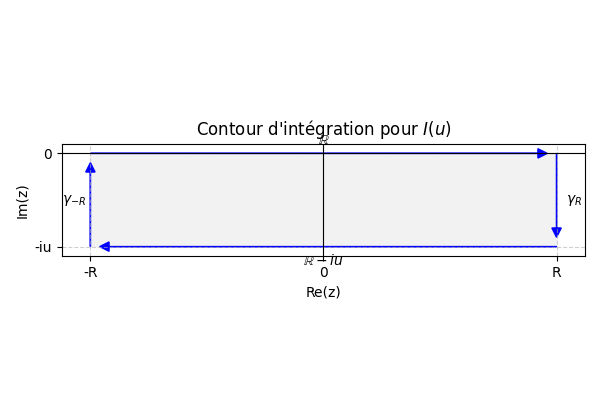
\includegraphics[width=0.6\textwidth]{contour_integration.png}
\caption{The rectangular contour in the complex plane used to show that $I(u)$ is constant.}
\label{fig:contour}
\end{figure}
Another method is to differentiate under the integral sign. Let $f(x, u) = e^{-\frac{1}{2}(x-iu)^2}$. We have $\frac{\partial f}{\partial u} = i(x-iu) e^{-\frac{1}{2}(x-iu)^2}$. This partial derivative is integrable with respect to $x$.
\begin{align*}
I'(u) = \int_{\mathbb{R}} \frac{\partial f}{\partial u}(x,u) dx &= \int_{\mathbb{R}} i(x-iu) e^{-\frac{1}{2}(x-iu)^2} dx \\
&= -i \int_{\mathbb{R}} \frac{\partial}{\partial x} \left( e^{-\frac{1}{2}(x-iu)^2} \right) dx \\
&= -i \left[ e^{-\frac{1}{2}(x-iu)^2} \right]_{-\infty}^{+\infty} = 0.
\end{align*}
Since $I'(u) = 0$, $I(u)$ is a constant. We can evaluate it at $u=0$:
\[ I(u) = I(0) = \int_{-\infty}^{+\infty} e^{-x^2/2} dx = \sqrt{2\pi}. \]
Thus, for $Z \sim \mathcal{N}(0,1)$,
\[ \varphi_Z(u) = e^{-u^2/2} \frac{1}{\sqrt{2\pi}} I(u) = e^{-u^2/2} \frac{\sqrt{2\pi}}{\sqrt{2\pi}} = e^{-u^2/2}. \]
Now, for $X \sim \mathcal{N}(m, \sigma^2)$, we have $X = \sigma Z + m$. Using the affine transformation property:
\[ \varphi_X(u) = \varphi_{\sigma Z + m}(u) = e^{ium} \varphi_Z(\sigma u) = e^{ium} e^{-(\sigma u)^2/2} = e^{ium - \frac{\sigma^2 u^2}{2}}. \]
%  \subsection{}
\end{example}% --- CHUNK_METADATA_START ---
% src_checksum: 85136617fd59de1773f414792722c11aedb2a74e5023e34b6205c03caa7ca4da
% needs_review: True
% --- CHUNK_METADATA_END ---
We note that the Gaussian density is an eigenvector of the Fourier transform.
Let $\psi_\sigma(x) = \frac{1}{\sqrt{2\pi}\sigma} e^{-x^2/(2\sigma^2)}$. We have $\int e^{iux} \psi_\sigma(x) dx = e^{-\sigma^2 u^2/2}$. By setting $g_{1/\sigma}(u) = e^{-u^2/(2/\sigma^2)}$, we have $\int e^{iux} \psi_\sigma(x) dx = \psi_{1/\sigma}(u)$.\\% --- CHUNK_METADATA_START ---
% src_checksum: 869df475c58a509f48611f7c6bc686e16c5897fa38b1872164541710dd0b987d
% needs_review: True
% --- CHUNK_METADATA_END ---
\subsection{Summary}% --- CHUNK_METADATA_START ---
% src_checksum: d6eb719c6effddf0612d89536e9b2f986a456e66231e44cbd7ebd2f667d70c12
% needs_review: True
% --- CHUNK_METADATA_END ---
The following table summarizes the characteristic features for several classical probability distributions.% --- CHUNK_METADATA_START ---
% src_checksum: 8643ccb27a58623bbf1940d0f2e5b874aecf902d3005145c1f9a14111a8e5e21
% needs_review: True
% --- CHUNK_METADATA_END ---
\begin{table}[H]
\centering
\begin{tabular}{|l|c|}
\hline
\textbf{Distribution} $P_X$ & $\varphi_X(u)$ \\
\hline
Dirac distribution$\delta_a$ & $e^{iau}$ \\
Bernoulli distribution$Ber(p)$ & $1-p+pe^{iu}$ \\
Poisson distribution$P(\lambda)$ & $\exp(\lambda(e^{iu}-1))$ \\
Geometric distribution$Geo(p)$ & $\frac{pe^{iu}}{1-(1-p)e^{iu}}$ \\
Exponential distribution$Exp(\alpha)$ & $\frac{\alpha}{\alpha - iu}$ \\
Uniform distribution$U(a,b)$ & $\frac{e^{iub}-e^{iua}}{iu(b-a)}$ \\
Normal distribution$N(m, \sigma^2)$ & $\exp\left(ium - \frac{1}{2}\sigma^2 u^2\right)$ \\
\hline
\end{tabular}
\caption{Characteristic functions of common distributions.}
\end{table}% --- CHUNK_METADATA_START ---
% src_checksum: 3f66216a725a4c16582ef0a683c2e58477e2829c4ca7fe1e2d7b0d2afa807af2
% needs_review: True
% --- CHUNK_METADATA_END ---
\section{Injectivity Theorem}% --- CHUNK_METADATA_START ---
% src_checksum: 1313ec4caa2b6959e0d5a779ab3b85d5345fb15417e8f21716739a45b928fbd5
% needs_review: True
% --- CHUNK_METADATA_END ---
\begin{theorem}
Let $\mathcal{M}_1(\mathbb{R})$ be the set of probability measures on $(\mathbb{R}, \mathcal{B}(\mathbb{R}))$. The mapping
\[ \mu \in \mathcal{M}_1(\mathbb{R}) \mapsto \varphi_{\mu} \]
is injective.
\end{theorem}% --- CHUNK_METADATA_START ---
% src_checksum: 2f9218124bb63c33f5b753b524b152c4059c9df42661f97f5a07e9e498954ae4
% needs_review: True
% --- CHUNK_METADATA_END ---
This fundamental theorem means that the characteristic function uniquely determines the probability law. If two random variables have the same characteristic function, they have the same law.% --- CHUNK_METADATA_START ---
% src_checksum: 85df9a18aea8f2f7361755c6d179993cdea9e6a0aef4d6e5b3b10573f368cabb
% needs_review: True
% --- CHUNK_METADATA_END ---
\begin{proof}[Idée de la preuve]
The idea is to show that the law of $X$ is determined by the family of laws of $X+\sigma Y$ for $\sigma > 0$, where $Y \sim \mathcal{N}(0,1)$ is independent of $X$. The law of $X+\sigma Y$ is a "regularized" (convolved) version of the law of $X$.
Let $(\Omega, \mathcal{F}, P)$ be a probability space on which two independent random variables are defined: $X \sim \mu$ and $Y \sim \mathcal{N}(0,1)$. For $\sigma > 0$, we study the variable $X_\sigma = X+\sigma Y$.
The characteristic function of $X_\sigma$ is:
\[ \varphi_{X_\sigma}(t) = E[e^{it(X+\sigma Y)}] = E[e^{itX}]E[e^{it\sigma Y}] = \varphi_X(t) \varphi_{\sigma Y}(t) = \varphi_\mu(t) e^{-\frac{\sigma^2 t^2}{2}}. \]
This function is determined by $\varphi_\mu(t)$.
Let $f: \mathbb{R} \to \mathbb{R}$ be a continuous function with compact support. The expectation $E[f(X+\sigma Y)]$ is given by:
\begin{align*}
E[f(X+\sigma Y)] &= \iint_{\mathbb{R}^2} f(x+\sigma y) d\mu(x) dP_Y(y) \\
&= \iint f(x+z) d\mu(x) g_\sigma(z) dz,
\end{align*}
where $g_\sigma(z)$ is the density of $\sigma Y \sim \mathcal{N}(0,\sigma^2)$.
Using the inverse Fourier representation for $f(z) = \frac{1}{2\pi} \int e^{-izt} \hat{f}(t) dt$, where $\hat{f}(t) = \int e^{izt}f(z)dz$ (Fourier transform convention), we can show that $E[f(X+\sigma Y)]$ is completely determined by $\varphi_\mu$. A more direct derivation (as seen in the notes) is as follows:
\begin{align*}
E[f(X+\sigma Y)] &= \iint f(x+y') d\mu(x) g_\sigma(y') dy' \\
\text{change of variable } z &= x+y' \\
&= \iint f(z) g_\sigma(z-x) d\mu(x) dz \\
&= \int f(z) \left( \int g_\sigma(z-x) d\mu(x) \right) dz.
\end{align*}
The inner integral is the density of the law of $X+\sigma Y$, which is the convolution of the measure $\mu$ and the Gaussian density $g_\sigma$. Since the Fourier transform of a convolution is the product of the Fourier transforms, the law of $X+\sigma Y$ has the characteristic function $\varphi_\mu(t) e^{-\sigma^2 t^2/2}$.
Since the characteristic function determines the law, the law of $X+\sigma Y$ is uniquely determined by $\varphi_\mu$.
Now, let $\sigma \to 0$. The random variable $X+\sigma Y$ converges in probability to $X$.
Indeed, for all $\epsilon > 0$:
\[ P(|(X+\sigma Y) - X| > \epsilon) = P(|\sigma Y| > \epsilon) = P\left(|Y| > \frac{\epsilon}{\sigma}\right). \]
When $\sigma \to 0$, $\frac{\epsilon}{\sigma} \to +\infty$. Therefore,
\[ \lim_{\sigma \to 0} P\left(|Y| > \frac{\epsilon}{\sigma}\right) = P(|Y| = \infty) = 0. \]
Thus, $X+\sigma Y \xrightarrow{P} X$.
Convergence in probability implies convergence in law: $X+\sigma Y \xrightarrow{d} X$.
Since the law of $X+\sigma Y$ is determined by $\varphi_\mu$ for all $\sigma>0$, its limit in law, which is the law of $X$, is also determined by $\varphi_\mu$. This proves injectivity.
The convergence in law ($X_n \xrightarrow{d} X$) is equivalent to the convergence of the distribution functions $F_{X_n}(x) \to F_X(x)$ for all points $x$ where $F_X$ is continuous. This can be shown by the following inequalities.
Let $x$ be a continuity point of $F_X$. For all $\epsilon > 0$:
\[ P(X_n \le x) \le P(|X_n - X| \ge \epsilon) + P(X \le x+\epsilon). \]
By taking the limit supremum as $n \to \infty$, and knowing that $X_n \xrightarrow{P} X$ (which implies $P(|X_n - X| \ge \epsilon) \to 0$), we obtain
\[ \limsup_{n\to\infty} F_{X_n}(x) \le F_X(x+\epsilon). \]
Similarly,
\[ P(X \le x-\epsilon) \le P(|X_n - X| \ge \epsilon) + P(X_n \le x). \]
By taking the limit infimum, we obtain
\[ F_X(x-\epsilon) \le \liminf_{n\to\infty} F_{X_n}(x). \]
Combining these two, for a continuity point $x$ of $F_X$, we can let $\epsilon \to 0$:
\[ F_X(x) \le \liminf_{n\to\infty} F_{X_n}(x) \le \limsup_{n\to\infty} F_{X_n}(x) \le F_X(x), \]
which proves that $\lim_{n\to\infty} F_{X_n}(x) = F_X(x)$.
\end{proof}